
\documentclass[12pt]{article}
\usepackage[greek,english]{babel}
\usepackage[utf8]{inputenc}
\usepackage{johd}

\usepackage{amssymb}
\usepackage{physics}
\usepackage{hyperref}


\title{Algorithmic Game Theory}

\author{Francesca Murano, Paola Guarasci  \\
        \small Department of Mathematics and Computer Science, \\
        \small University of Calabria\\
}
\begin{document}
\maketitle
\begin{center}
    \textbf{University Project}
\end{center}

\section*{Research Objective}
 \
{Define a system that can choose a number of users to take a tour. The number of users and the maximum number of kilometers that can be traveled is fixed. Each user has a budget that they cannot exceed. The costs of the tour are divided into proportional costs related to the distance of the tour and fixed costs.
}


\section*{Outline}
\begin{itemize}
    \item[1.] Bayesian Game Settings
    \item [2.] Quasilinear mechanism
    \item[2.1.] Direct quasilinear mechanism
    \item[3.] Vickrey-Clarke-Groves Mechanisms
    \item[4.] Problem Resolution
\end{itemize}
\newpage

\section{Bayesian Game Settings}   
A Bayesian game is a type of game in which players have \textbf{incomplete information} about the other players' characteristics or strategies. In this game, each player has a prior belief about the distribution of the other players' types.

The main challenge in a Bayesian game is to find a strategy that maximizes a player's expected \textbf{utility} given their prior beliefs about the other players. 
They are called Bayesian because of the probabilistic analysis inherent in the game. 

A Bayesian game is a tuple (N,O,$\Theta$,p,u), where:
\begin{itemize}
    \item N = \{1,...,n\} is a finite set of players; \\
    \item O = a set of outcomes;\\
    \item $\Theta$ = $\theta$\textsubscript{1} × ··· × $\theta$\textsubscript{n}, with $\theta$\textsubscript{i} the set of possible types of player i; \\
    \item p : $\Theta$$\rightarrow$[0,1] is the probability distribution over $\Theta$; \\
    \item u = (u\textsubscript{1},...,u\textsubscript{n}) is a profile of utility functions u\textsubscript{i} : A × $\Theta \rightarrow R$. 
\end{itemize}

\section{Quasilinear Mechanism}
A mechanism in the quasilinear setting is a triple (A, $\chi$ ,$\mathcal{P}$), where:
\begin{itemize}
    
    \item  A = A\textsubscript{1} × · · · × A\textsubscript{n}, where A\textsubscript{i} is the set of actions available to agent i $\in$ N;

    \item x : A $\rightarrow \Pi(X)$ maps each action profile to a distribution over choices;
    
     \item  $\mathcal{P}$: A $\rightarrow R ^{n}$ maps each action profile to a payment for each agent.
     
 \end{itemize}
 The use of a quasilinear mechanism came about because its strengths:
\begin{itemize}
\item the mechanism can choose to charge or reward agents with an arbitrary monetary amount, so our users can choose their own budget;

\item an agent's degree of preference for selecting \textbf{any choice is independent} of the amount.
So our users will choose the destination of the trip just for pleasure without thinking about the amount needed.  
This feature is really important as it leads users to focus only on their own interests without seeking strategies based on others' choices. They have no need to lie and always proclaim the truth.
\end{itemize}
\subsection{Direct quasilinear mechanism}
A direct quasilinear mechanism is a pair ($\chi$,$\wp$). It defines a mechanism in the quasilinear setting, where for each i, A\textsubscript{i} = $\Theta$\textsubscript{i}.
The set of actions available to each player is just the set of possible preferences of the player.
\newpage
\section{Vickrey-Clarke-Groves Mechanisms}
For the problem resolution, the choice fell on a mechanism belonging to the \textbf{Groves mechanisms}. Groves mechanisms belong to the direct quasilinear mechanisms ($\chi$,$\wp$),for which:

\begin{itemize}
\centering
    \item $\mathrm{\chi({\hat{v}}) = arg max_x\sum_{i}^n v_i(x)}$;  

    \item $\mathrm{\wp_i({\hat{v}})} = h_i(\hat{v}\textsubscript{-i}) - \sum_{i\neq j}^n \hat{v}_j(\chi(\hat{v}))$;\par
    
\end{itemize}

The dominant strategy of the mechanism is \textbf{truthtelling}, this mechanism allows us to make efficient choices.
\begin{center}
    \textbf{What does it mean efficiency?\\}
\end{center} 

A quasilinear mechanism is efficient, if in equilibrium it selects a choice $x$ such that:
\centering
\vspace*{ 10 mm}

$\forall{v}\forall{x'}$,$\quad\sum_{i=0}$$^n_i v_i(x)$
$\quad\geq$$\quad\sum_{i=0}$$^n_i \quad v_i(x')$ \\
\vspace*{8 mm} 

In VCG mechanism, h$_i$ is replace with:

\begin{itemize}
\centering
    \item $h_i$($\hat{v}_i$) 
=     $\sum_{i\neq j}^n$$\hat{v}_j$
        ($\chi$($\hat{v}$\textsubscript{$-i$}))
\end{itemize}
\hfill 
\newline
Using this information, it is possible now to establish how the VCG mechanism is structured:

\begin{itemize}
\centering
\item $\chi$($\hat{v}$) = arg max$_x$$\sum_{i}^n v_i(x)$;
\item $\wp_i(\hat{v}$) = $\sum_{i\neq j}^n$ $\hat{v}$$_j$($\chi$($\hat{v}\textsubscript{$-i$}))$$-$
$\sum_{i\neq j}^n$ $\hat{v}$$_j$
($\chi$($\hat{v}$));
\end{itemize}
\newpage
\begin{flushleft}
\section{Problem Resolution}
\textbf{Goal:} Organize a travel composed by k players following some rules:
\end{flushleft}

\begin{itemize}
    \item each player has a budget;
    \item each player is an agent represented by an arc;
    \item each player has fixed and variables costs proportional to travel length;
    \item each player declares truthfully its interests;
    \item the bus has a fixed number of places;
    \item the tour start and finish in the same place;
    \item the bus has maximum number of km that can be covered;
\end{itemize}
\begin{flushleft}
\subsection{Definition of variables}
\end{flushleft}
\begin{itemize}
    \item P :- set of total players;
    \begin{center}
        P = \{Francesca, Paola\}\
    \end{center}
    \item S :- subset of players joining the travel;\
    \begin{center}
        S = \{S $\subseteq$ P: $\abs{S}$ = k\}\ , k is the number of players;

    \end{center}
     \item L :- set of locations available;\
    \begin{center}
        L = \{Genoa, Milan, Turin\}\ 

\end{center}
\end{itemize}
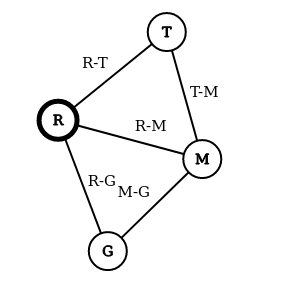
\includegraphics[width=0.4\columnwidth]{images/graph.png}

\end{document}